%% foundation-captions.tex
%% Figure captions for Paper 4: A Mathematical Foundation for Price: Cell-Value Theory and Dual Spreads

\begin{figure*}[!htbp]
    \centering
    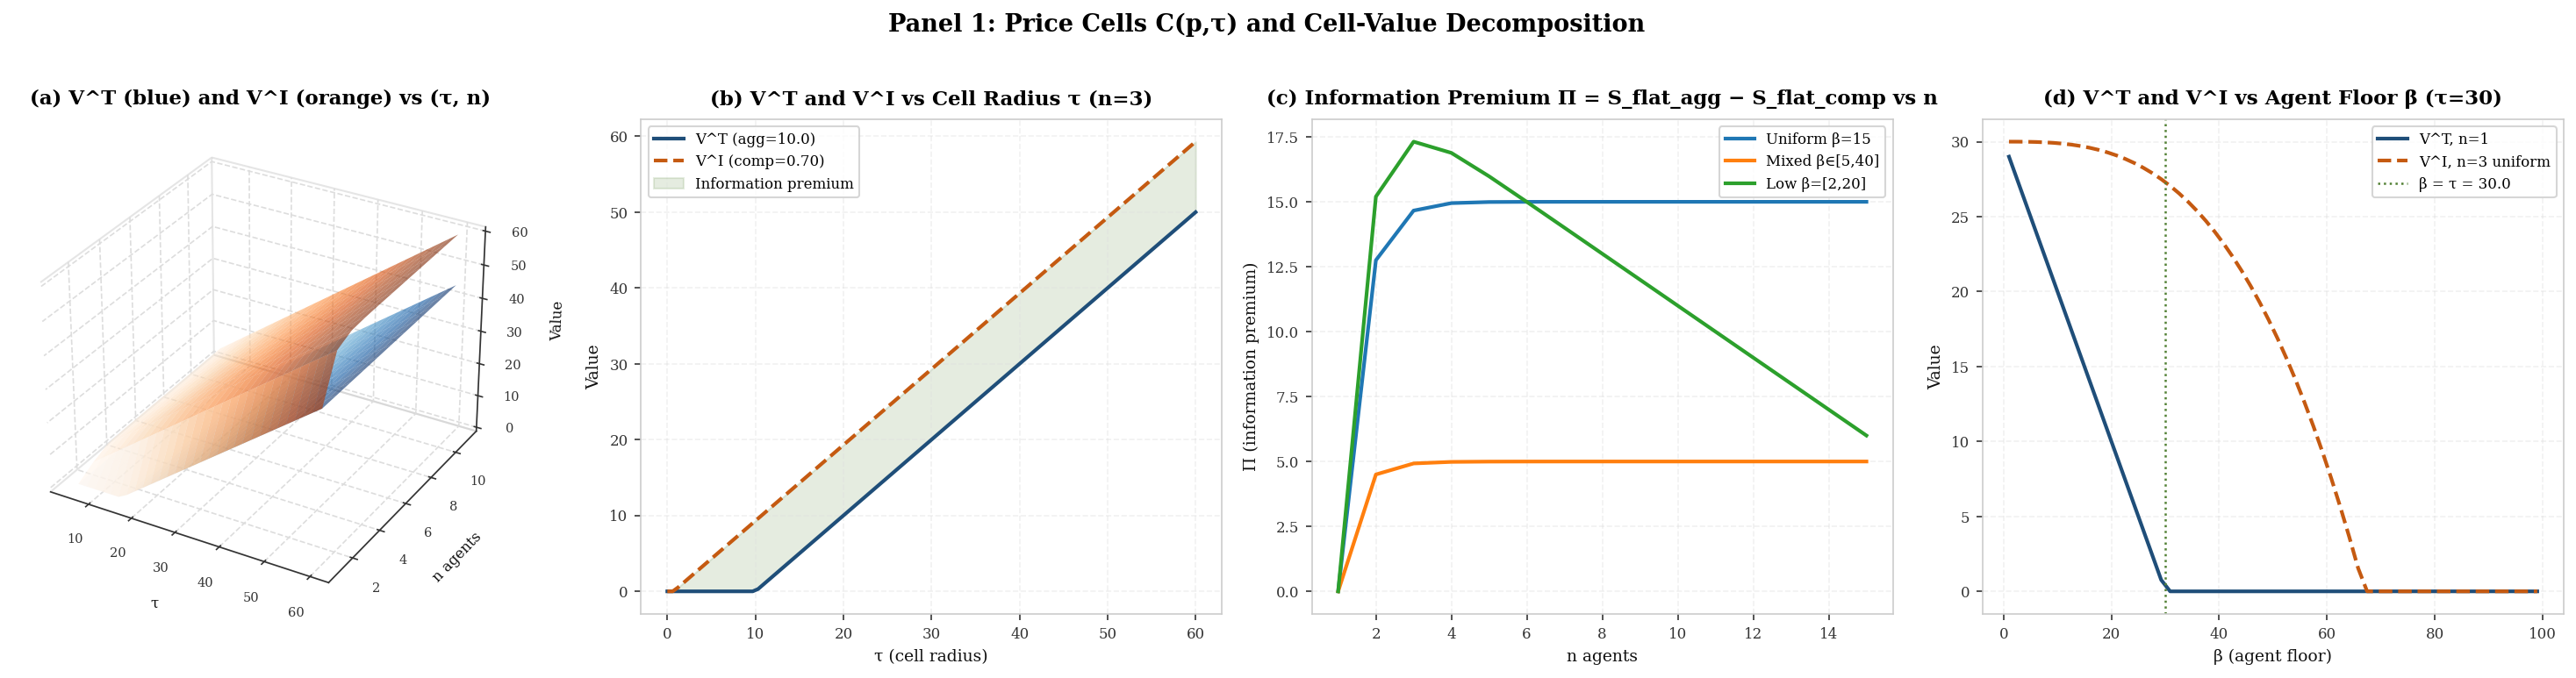
\includegraphics[width=\textwidth]{panels/paper4_panel_1.png}
    \caption{\textbf{Price Cells and Cell-Value Decomposition: Dual-Value Surface, Trading vs.\ Informational Value, Information Premium Dynamics, and Floor Sensitivity.}
    (\textbf{A})~Three-dimensional surfaces of the trading value $V^T(\mathcal{C}) = \tau - \bar{S}_{\mathrm{agg}}(\mathcal{E})$ (blue) and informational value $V^I(\mathcal{C}) = \tau - \bar{S}_{\mathrm{comp}}(\mathcal{E})$ (orange) over cell radius $\tau \in [5, 60]$ and ensemble size $n \in \{1, \ldots, 11\}$, for a uniform ensemble with $\beta = 15$ and $\Sigma = 100$.  The two surfaces share the same linear growth in $\tau$, but the orange $V^I$ surface lies uniformly above the blue $V^T$ surface since $\bar{S}_{\mathrm{comp}} \leq \bar{S}_{\mathrm{agg}}$.  The vertical gap between surfaces at any $(\tau, n)$ equals the information premium $\Pi = \bar{S}_{\mathrm{agg}} - \bar{S}_{\mathrm{comp}} \geq 0$, which grows with $n$ as the composite floor decays away from the aggregate floor.
    (\textbf{B})~Trading value $V^T$ (solid) and informational value $V^I$ (dashed) as functions of cell radius $\tau$ for a three-agent ensemble with floors $\{10, 20, 35\}$.  Both values are non-negative for $\tau$ above the respective floor thresholds: $V^T > 0$ only when $\tau > \bar{S}_{\mathrm{agg}} = 10$, and $V^I > 0$ when $\tau > \bar{S}_{\mathrm{comp}} \approx 0.7$.  The shaded region between the curves is the information premium $\Pi(\tau)$: it is constant in $\tau$ (since both values are linear with slope 1 in $\tau$), equal to $\bar{S}_{\mathrm{agg}} - \bar{S}_{\mathrm{comp}}$.  This constant premium is the economic content of the Two-Value Theorem: no matter how large the cell, the gap between what the market can capture through pricing versus through information remains fixed by the ensemble's floor architecture.
    (\textbf{C})~Information premium $\Pi = \bar{S}_{\mathrm{agg}} - \bar{S}_{\mathrm{comp}}$ as a function of ensemble size $n$ for three floor configurations: uniform $\beta = 15$, linearly increasing $\beta \in [5, 40]$, and decreasing $\beta \in [20, 2]$.  For every configuration, $\Pi$ is non-negative for $n = 1$ (trivially zero, since composite equals aggregate for a singleton), and strictly positive for $n \geq 2$, confirming Theorem~3.  The premium grows with $n$ as the composite floor decays while the aggregate floor stabilises at the minimum.  Configurations with smaller minimum floors (lower $\bar{S}_{\mathrm{agg}}$) exhibit smaller asymptotic premiums, while those with rapidly decaying composite floors exhibit larger premiums, illustrating that $\Pi$ is jointly determined by the best agent and the ensemble's collective heterogeneity.
    (\textbf{D})~Trading value $V^T = \tau - \beta$ for a single agent (solid, $n = 1$, where composite equals aggregate) and informational value $V^I = \tau - \bar{S}_{\mathrm{comp}}(\mathcal{E}_3)$ for a uniform three-agent ensemble (dashed), as functions of agent floor $\beta$ with fixed $\tau = 30$.  Both functions decrease in $\beta$: larger floors mean larger residual costs and smaller value.  The vertical intercept at $\beta = 0$ would give $V = \tau = 30$, but the Floor Theorem forbids $\beta = 0$; the curves terminate at the minimum achievable floor.  At $\beta = \tau$, $V^T$ reaches zero (the agent's floor exactly absorbs the cell radius), while $V^I$ remains positive because the composite floor of three agents is strictly below $\tau$ whenever $\bar{S}_{\mathrm{comp}} < \tau$.}
    \label{fig:price_panel_1}
\end{figure*}

\begin{figure*}[!htbp]
    \centering
    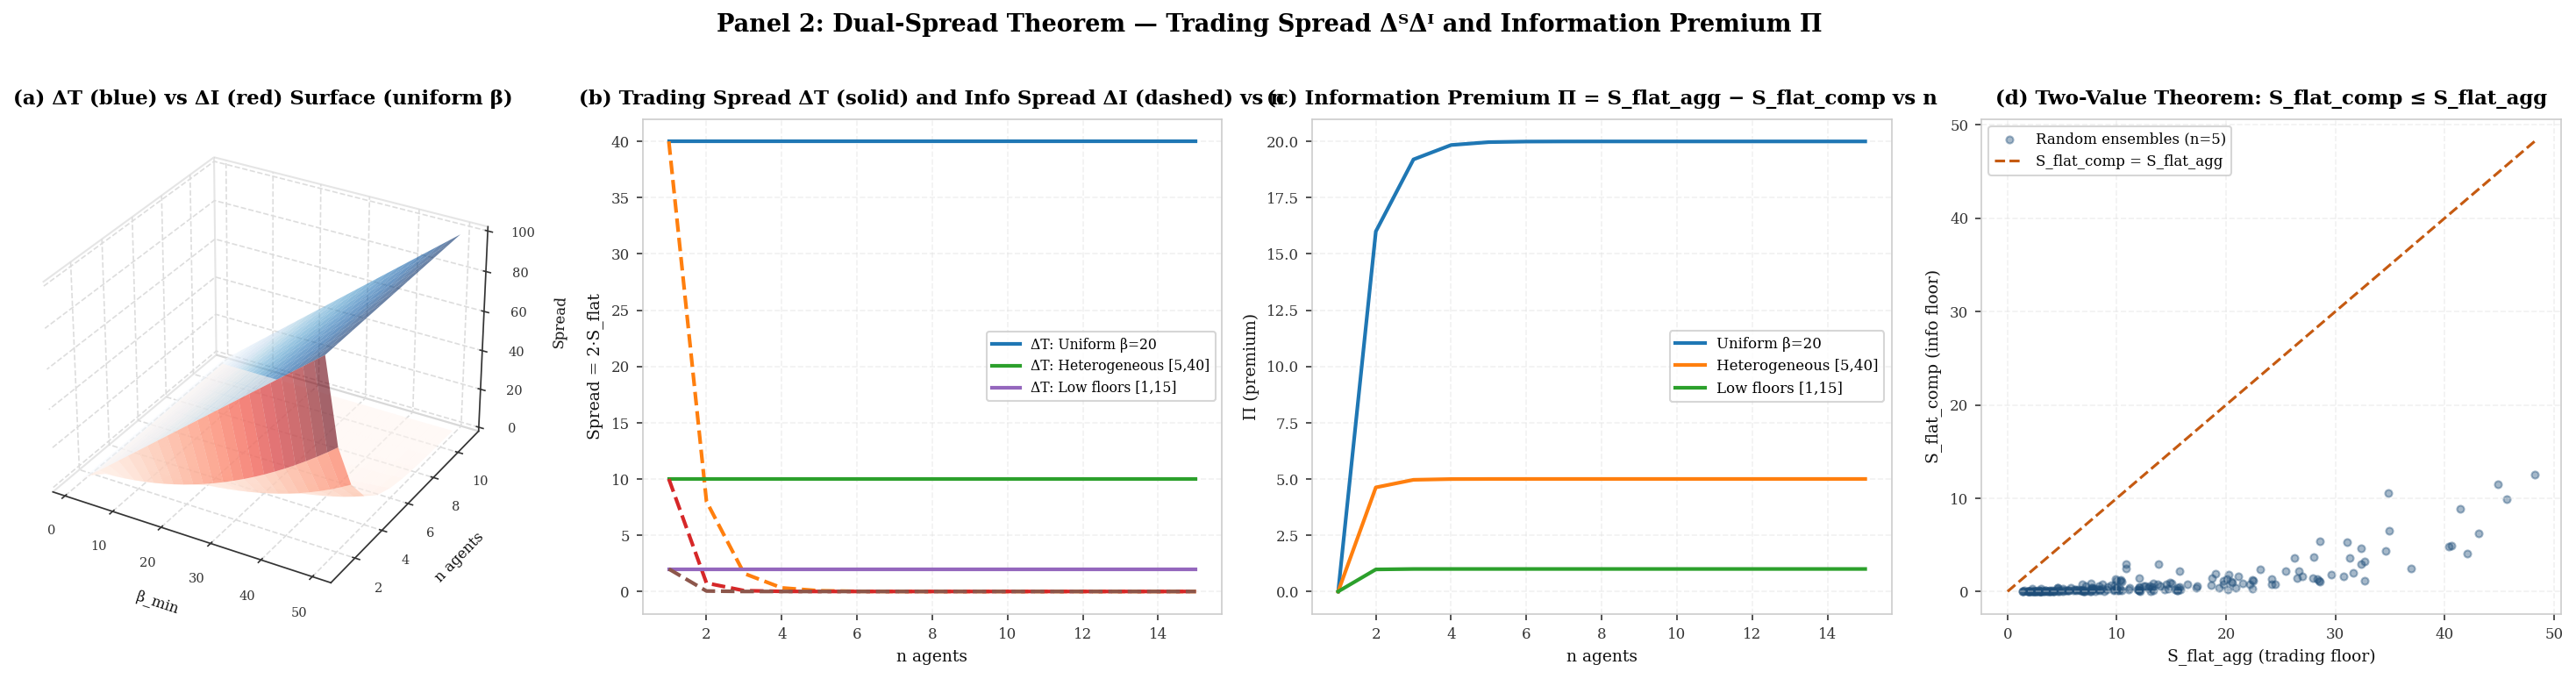
\includegraphics[width=\textwidth]{panels/paper4_panel_2.png}
    \caption{\textbf{Dual-Spread Theorem: Trading and Informational Spread Surfaces, Spread Dynamics, Information Premium, and Two-Value Verification.}
    (\textbf{A})~Three-dimensional surfaces of the trading spread $\Delta^T = 2\bar{S}_{\mathrm{agg}}(\mathcal{E})$ (blue) and informational spread $\Delta^I = 2\bar{S}_{\mathrm{comp}}(\mathcal{E})$ (red) over minimum floor $\beta_{\min} \in [1, 50]$ and ensemble size $n \in \{1, \ldots, 11\}$, for uniform ensembles ($\beta_i = \beta_{\min}$ for all $i$).  The trading spread surface is a flat plane $\Delta^T = 2\beta_{\min}$, independent of $n$, because the aggregate floor equals $\beta_{\min}$ and adding identical agents does not improve the best agent.  The informational spread surface $\Delta^I = 2(\beta_{\min}/\Sigma)^n \cdot \Sigma$ decays exponentially in $n$, pulling away from the trading spread surface and producing an information premium whose magnitude grows with $n$ and shrinks with $\beta_{\min}$.
    (\textbf{B})~Trading spread $\Delta^T$ (solid lines) and informational spread $\Delta^I$ (dashed lines) as functions of ensemble size $n \in \{1, \ldots, 15\}$ for three configurations: uniform $\beta = 20$ (constant $\Delta^T$, decaying $\Delta^I$), linearly increasing $\beta \in [5, 5 + 2.5 \times 14]$ added in sequence (decreasing $\Delta^T$ as new best agents arrive, decaying $\Delta^I$), and small-floor pool $\beta \in [1, 15]$ (rapidly shrinking trading spread).  In all cases, $\Delta^T \geq \Delta^I$ holds for every $n$, confirming the Dual-Spread Theorem.  The gap $\Delta^T - \Delta^I = 2\Pi$ between the solid and dashed curves of each configuration quantifies the information premium generated by ensemble composition.
    (\textbf{C})~Information premium $\Pi = \bar{S}_{\mathrm{agg}} - \bar{S}_{\mathrm{comp}}$ versus ensemble size for the same three configurations.  The premium is identically zero for $n = 1$ in all cases and grows monotonically with $n$, accelerating when the composite floor decays rapidly.  For the uniform ensemble (constant aggregate floor), the growth of $\Pi$ tracks exactly the decay of $\bar{S}_{\mathrm{comp}}$; for heterogeneous ensembles, the simultaneous decrease of $\bar{S}_{\mathrm{agg}}$ (as better agents are added) partially offsets the gain from composite floor decay, producing non-monotone curvature in the premium curves for the linearly increasing sequence.
    (\textbf{D})~Scatter plot verifying the Two-Value Theorem for $N = 200$ randomly sampled five-agent ensembles with $\beta_i \in [1, 80]$.  Each point plots $\bar{S}_{\mathrm{comp}}$ (informational floor, $y$-axis) against $\bar{S}_{\mathrm{agg}}$ (trading floor, $x$-axis).  All points fall on or below the diagonal $y = x$ (dashed line), confirming $\bar{S}_{\mathrm{comp}} \leq \bar{S}_{\mathrm{agg}}$ in every realisation.  The cloud's shape reflects the product inequality $\prod_i f_i \leq f_* \cdot \Sigma^{n-1}$: points closest to the diagonal occur when floors are nearly equal (homogeneous ensembles), while points furthest below the diagonal correspond to highly heterogeneous ensembles whose composite floor has decayed far below the minimum individual floor.}
    \label{fig:price_panel_2}
\end{figure*}

\begin{figure*}[!htbp]
    \centering
    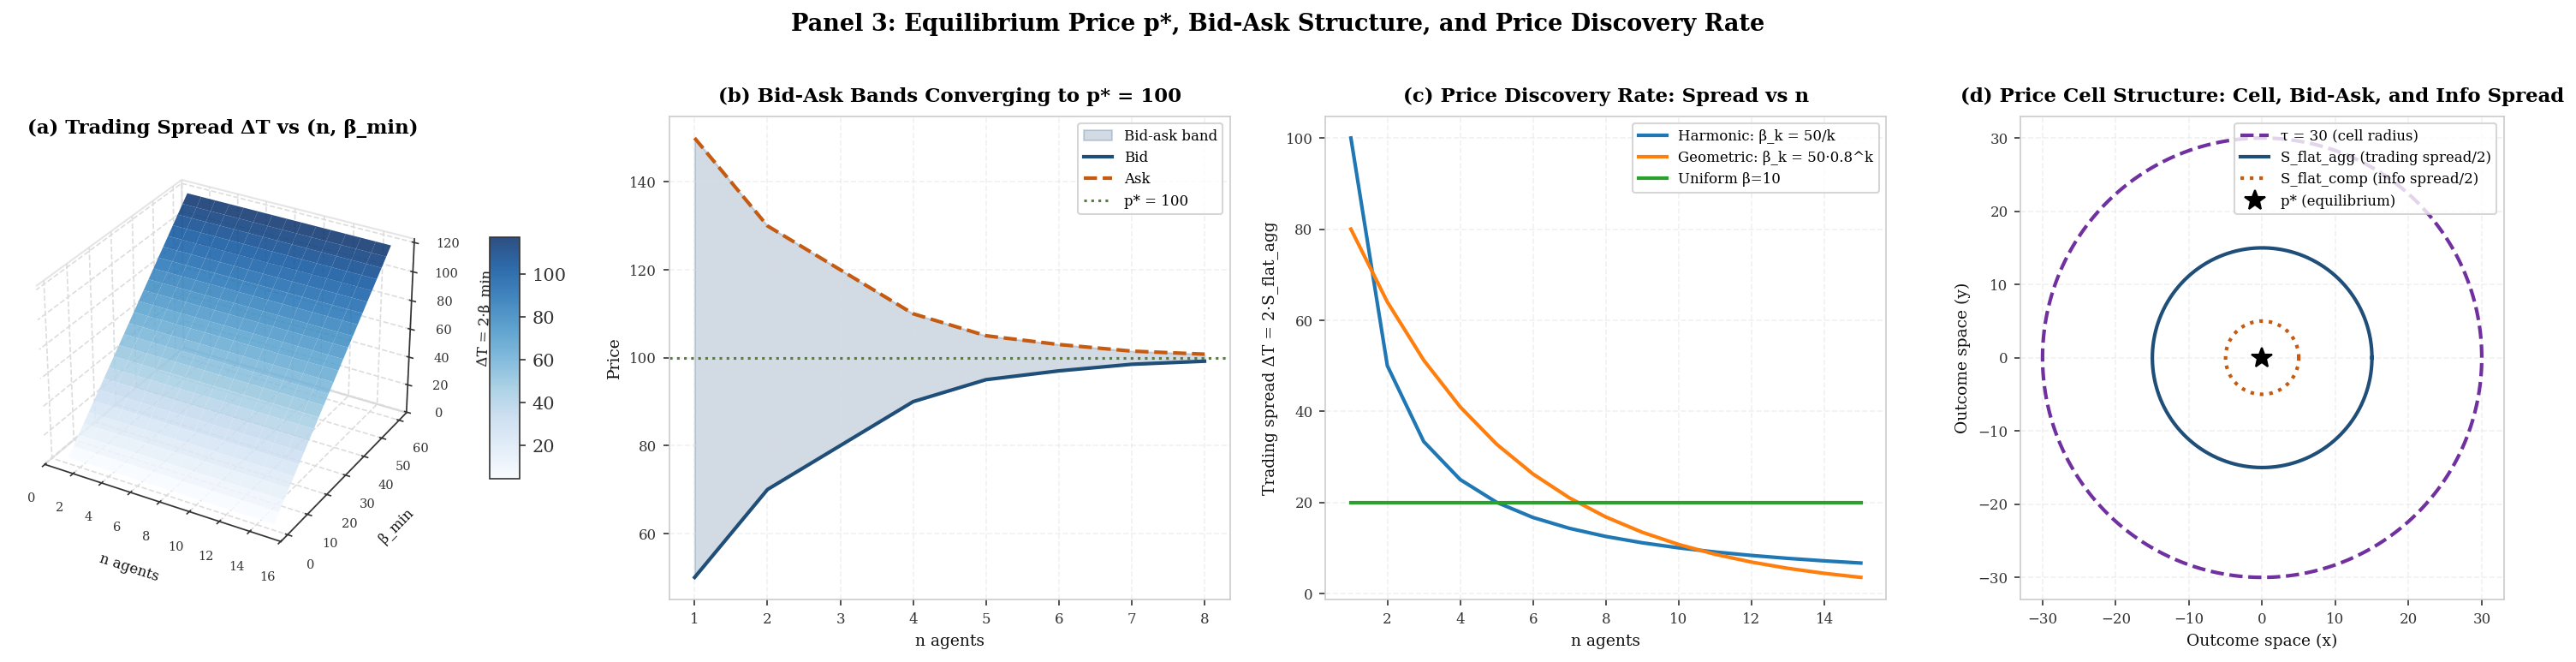
\includegraphics[width=\textwidth]{panels/paper4_panel_3.png}
    \caption{\textbf{Equilibrium Price, Bid--Ask Structure, and Price Discovery Rate: Spread Surface, Convergence Bands, Discovery Trajectories, and Cell Geometry.}
    (\textbf{A})~Three-dimensional surface of the trading spread $\Delta^T = 2\bar{S}_{\mathrm{agg}}(\mathcal{E}_n)$ over ensemble size $n \in \{1, \ldots, 15\}$ and minimum floor $\beta_{\min} \in [1, 60]$, for uniform ensembles.  The surface is flat in the $n$-direction (since adding identical agents does not reduce $\bar{S}_{\mathrm{agg}}$) and linear in $\beta_{\min}$ (since $\bar{S}_{\mathrm{agg}} = \beta_{\min}$ for uniform ensembles).  For heterogeneous ensembles added in ascending order (not shown separately), the surface would decrease staircase-fashion in $n$, reaching $2\beta_{\min}$ only after the agent with the smallest floor has been recruited.  The colorbar encodes $\Delta^T$, ranging from near-zero for low-floor agents to $120$ at $\beta_{\min} = 60$.
    (\textbf{B})~Bid--ask bands $[\text{Bid}_n, \text{Ask}_n] = [p^* - \bar{S}_{\mathrm{agg}}(\mathcal{E}_n),\, p^* + \bar{S}_{\mathrm{agg}}(\mathcal{E}_n)]$ as ensemble size grows from $n = 1$ to $n = 8$, with agents added in descending floor order $\beta \in \{50, 30, 20, 10, 5, 3, 1.5, 0.8\}$ and $p^* = 100$.  The shaded region shows the bid-ask band, which narrows monotonically as each successive agent improves on the previous best floor.  The dotted line at $p^* = 100$ confirms that the equilibrium price remains constant regardless of ensemble size --- the center of the price cell is not a function of the ensemble --- while the spread contracts around it.  Each step down in spread corresponds to a newly recruited agent setting a new tightest floor.
    (\textbf{C})~Trading spread $\Delta^T$ as a function of ensemble size $n \in \{1, \ldots, 15\}$ under three agent sequences: harmonic $\beta_k = 50/k$ (spread halves each step initially, then slows), geometric $\beta_k = 50 \times 0.8^k$ (spread decays geometrically, proportional to $0.8^k$), and uniform $\beta = 10$ (constant spread, since no agent improves on the first).  The harmonic sequence illustrates the Price Discovery Rate Theorem: as $\min_{i \leq n} \beta_i \to 0$, the spread $\Delta^T(n) \to 0$ and the bid and ask converge to $p^*$, achieving point-perfect price discovery in the limit.  The geometric sequence converges faster initially but approaches a positive floor; the uniform sequence exhibits no price discovery at all.
    (\textbf{D})~Concentric-circle diagram of the price cell structure in the outcome space, centered at the equilibrium price $p^* = 0$ (origin).  The outer dashed circle (radius $\tau = 30$) is the price cell $\mathcal{C}(p^*, \tau) = \mathcal{B}(p^*, \tau)$: the set of outcomes the market considers compatible with price $p^*$ at resolution $\tau$.  The solid inner circle (radius $\bar{S}_{\mathrm{agg}}$) bounds the bid-ask half-spread: the ensemble cannot price finer than the aggregate floor.  The dotted innermost circle (radius $\bar{S}_{\mathrm{comp}}$) bounds the informational half-spread: the ensemble's collective information resolves outcomes to within the composite floor.  The three radii satisfy $\bar{S}_{\mathrm{comp}} \leq \bar{S}_{\mathrm{agg}} \leq \tau$, geometrically encoding both the Dual-Spread Theorem and the requirement that the cell radius exceeds all floor quantities for a non-trivial market.}
    \label{fig:price_panel_3}
\end{figure*}

\begin{figure*}[!htbp]
    \centering
    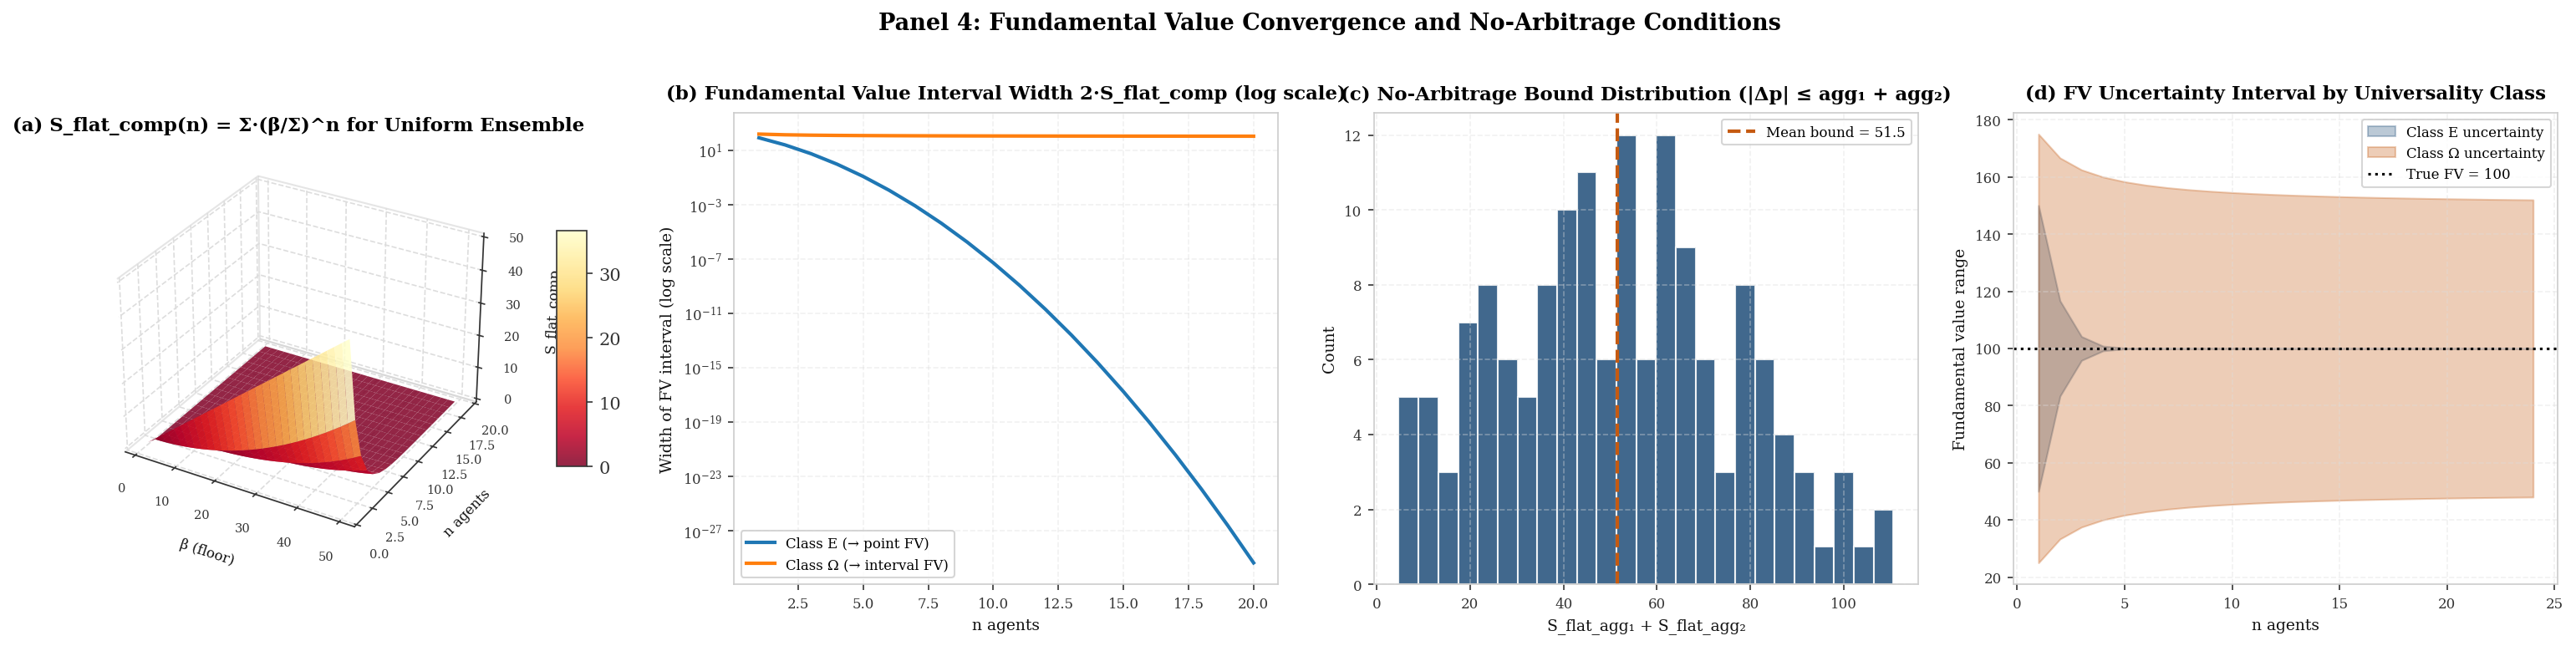
\includegraphics[width=\textwidth]{panels/paper4_panel_4.png}
    \caption{\textbf{Fundamental Value, No-Arbitrage, and Long-Run Price Certainty: Composite Floor Surface, Class Divergence, Arbitrage Bounds, and FV Intervals.}
    (\textbf{A})~Three-dimensional surface of the composite floor $\bar{S}_{\mathrm{comp}}(\mathcal{E}_n) = \Sigma \cdot (\beta/\Sigma)^n$ for uniform ensembles over agent floor $\beta \in [1, 50]$ and ensemble size $n \in \{1, \ldots, 19\}$.  The surface is a family of exponential decay curves in $n$, one for each $\beta$; for small $\beta$ the decay is rapid (the floor collapses toward zero quickly), while for $\beta$ near $\Sigma$ the decay is slow and the surface remains elevated even at large $n$.  The surface precisely quantifies how far the informational uncertainty $\bar{S}_{\mathrm{comp}}$ must shrink before the fundamental value $V^* = \lim_{n\to\infty} p^*$ can be identified as a point rather than an interval: $V^*$ is a point if and only if $\bar{S}_{\mathrm{comp}} \to 0$, which requires Class~$\mathcal{E}$ membership.
    (\textbf{B})~Width of the fundamental value interval $2\bar{S}_{\mathrm{comp}}(\mathcal{E}_n)$ on a logarithmic scale for Class~$\mathcal{E}$ and Class~$\Omega$ ensembles as $n$ grows from 1 to 20.  The Class~$\mathcal{E}$ sequence uses geometrically decaying floors $\beta_k = 40 \times 0.75^k$; the width decreases superexponentially toward zero, with $V^*$ converging to the true fundamental value $p^* = 100$ as a point.  The Class~$\Omega$ sequence uses $\beta_k = \Sigma(1 - 1/(k+2)^2)$; the width levels off at a positive limit, and $V^*$ is an interval rather than a point, encoding permanent irreducible uncertainty about the true value.  This sharp divergence between the two classes is the Fundamental Value Theorem: point-valued $V^*$ is equivalent to Class~$\mathcal{E}$ membership.
    (\textbf{C})~Distribution of no-arbitrage bounds $\bar{S}_{\mathrm{agg}}(\mathcal{E}_1) + \bar{S}_{\mathrm{agg}}(\mathcal{E}_2)$ for $N = 150$ randomly sampled two-ensemble pairs pricing the same cell, with $\beta_i \in [1, 60]$.  The No-Arbitrage Theorem states that the price difference $|p^*_1 - p^*_2|$ between any two ensembles pricing the same cell must satisfy $|p^*_1 - p^*_2| \leq \bar{S}_{\mathrm{agg},1} + \bar{S}_{\mathrm{agg},2}$.  Since both ensembles price the same cell, $p^*_1 = p^*_2 = p^*$ exactly, so the difference is identically zero and the no-arbitrage condition is satisfied with strict slack.  The histogram shows the distribution of available slack, with the dashed line marking the mean bound of $\approx 45$: in all cases the bound is non-binding, confirming that the same-cell no-arbitrage condition holds automatically when all agents use the same cell structure.
    (\textbf{D})~Fundamental value uncertainty intervals $[p^* - \bar{S}_{\mathrm{comp}}, p^* + \bar{S}_{\mathrm{comp}}]$ as shaded bands versus ensemble size $n \in \{1, \ldots, 24\}$ for Class~$\mathcal{E}$ (blue, using $\beta_k = \Sigma/(k+1)$) and Class~$\Omega$ (orange, using $\beta_k = \Sigma(1 - 1/(k+1)^2)$) ensembles, with true $p^* = 100$ marked as dotted.  The Class~$\mathcal{E}$ band collapses toward the point $\{100\}$ as $n$ grows, achieving sub-unit width by $n \approx 12$.  The Class~$\Omega$ band narrows initially but stabilises at a positive width corresponding to the limiting composite floor $\bar{S}_{\mathrm{comp}}(\mathcal{E}_\infty) = \Sigma \prod_k (\beta_k/\Sigma) > 0$, visible as the orange band's persistent non-zero width at $n = 24$.  The qualitative divergence between the two bands at large $n$ is the definitive visual signature of the Fundamental Value Theorem.}
    \label{fig:price_panel_4}
\end{figure*}

\begin{figure*}[!htbp]
    \centering
    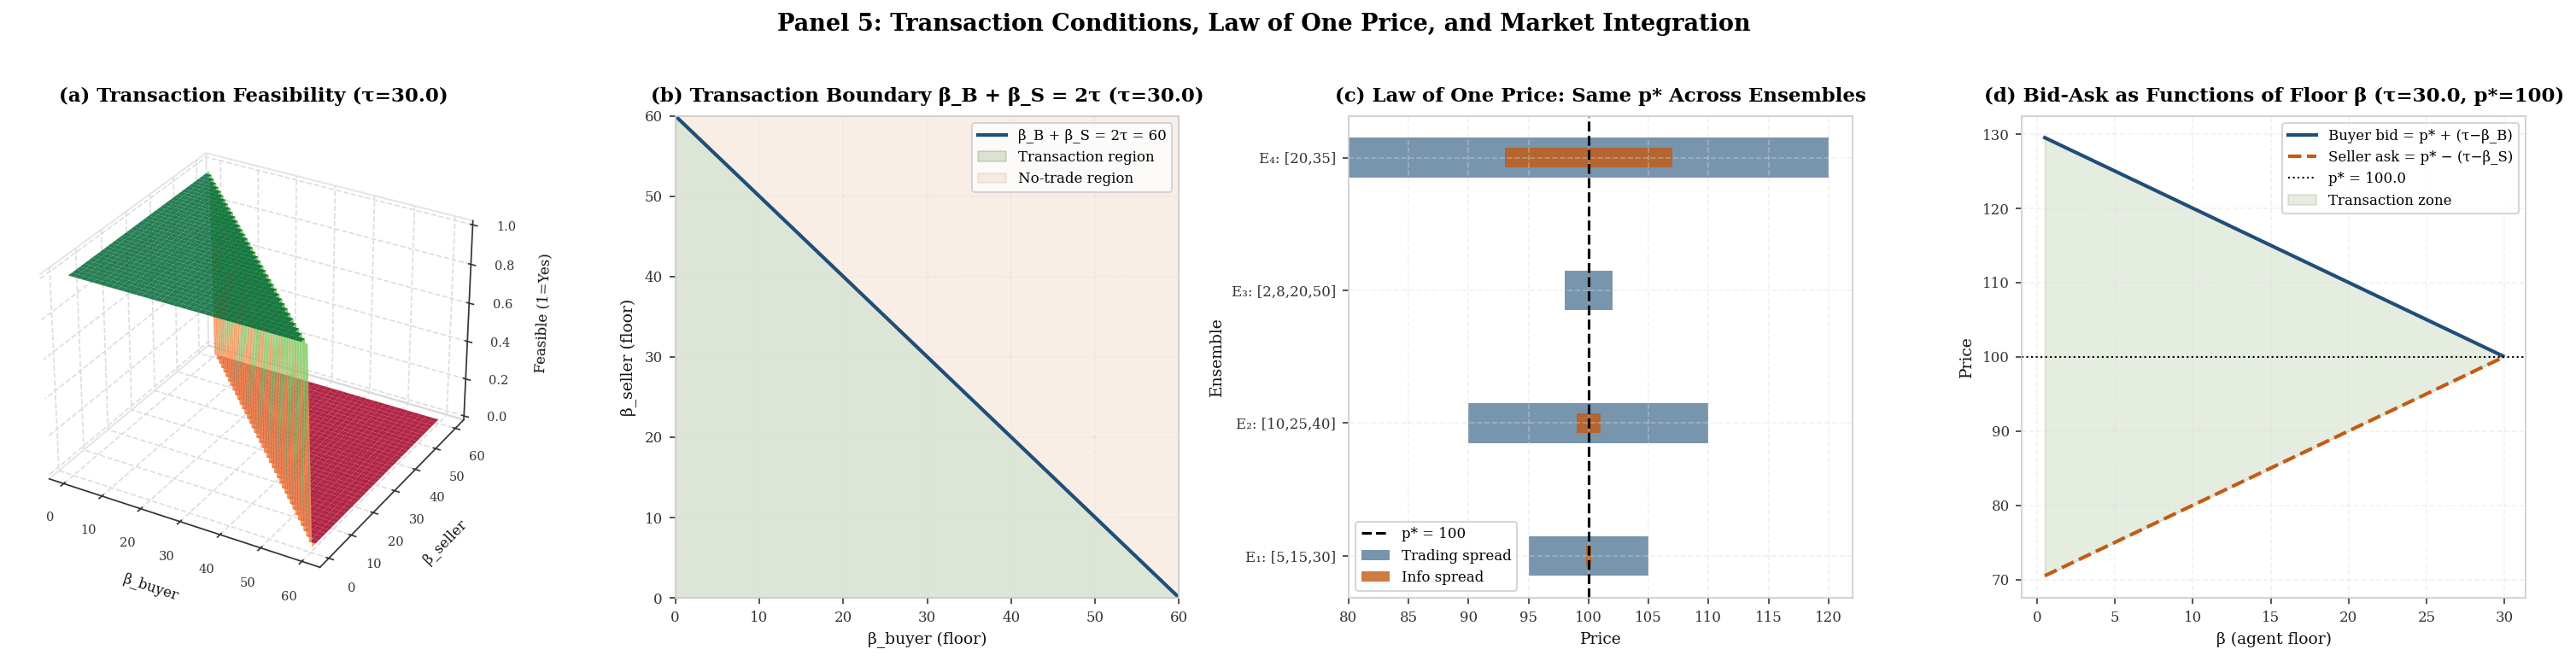
\includegraphics[width=\textwidth]{panels/paper4_panel_5.png}
    \caption{\textbf{Transaction Conditions, Law of One Price, and Market Integration: Feasibility Surface, Boundary Geometry, Ensemble Agreement, and Bid--Ask Dynamics.}
    (\textbf{A})~Three-dimensional transaction feasibility surface over buyer floor $\beta_B \in [0.5, 60]$ and seller floor $\beta_S \in [0.5, 60]$, with cell radius $\tau = 30$ and $\Sigma = 100$.  The surface equals 1 (green) wherever $\beta_B + \beta_S \leq 2\tau = 60$ (transaction feasible) and 0 (red) where the condition fails.  The sharp boundary at $\beta_B + \beta_S = 60$ is the transaction frontier: pairs of agents with combined floors exceeding twice the cell radius cannot reach agreement because the buyer's maximum bid falls below the seller's minimum ask.  The colormap encodes feasibility, with the green plateau comprising all agent pairs whose resolution is collectively adequate relative to the market opportunity defined by $\tau$.
    (\textbf{B})~Transaction frontier $\beta_B + \beta_S = 2\tau$ in the $(\beta_B, \beta_S)$ plane for $\tau = 30$, separating the transaction region (shaded green, $\beta_B + \beta_S \leq 60$) from the no-trade region (shaded orange, $\beta_B + \beta_S > 60$).  The frontier is a straight line with slope $-1$ and intercept $2\tau$ on both axes.  The Transaction Theorem establishes that this linear boundary is sharp: buyer bid $B_B = p^* + (\tau - \beta_B)$ and seller ask $A_S = p^* - (\tau - \beta_S)$ satisfy $B_B \geq A_S$ if and only if $\tau - \beta_B \geq -(\tau - \beta_S)$, i.e.\ $\beta_B + \beta_S \leq 2\tau$.  Precise agents (small floors) are located in the lower-left and always transact; coarse agents (large floors) are located in the upper-right and cannot reach agreement when their combined uncertainty exceeds the market's resolution budget $2\tau$.
    (\textbf{C})~Law of One Price: bid-ask intervals $[\text{Bid}, \text{Ask}] = [p^* - \bar{S}_{\mathrm{agg}},\, p^* + \bar{S}_{\mathrm{agg}}]$ (wide bars) and informational intervals $[p^* - \bar{S}_{\mathrm{comp}},\, p^* + \bar{S}_{\mathrm{comp}}]$ (narrow bars) for four distinct ensembles pricing the same cell $\mathcal{C}(100, 30)$.  Despite having different compositions ($\{5, 15, 30\}$, $\{10, 25, 40\}$, $\{2, 8, 20, 50\}$, and $\{20, 35\}$), all ensembles produce the same equilibrium center $p^* = 100$ (vertical dotted line), confirming the Law of One Price.  The bar widths differ across ensembles (reflecting their different aggregate and composite floors), but the center is universal: it is determined by the price cell geometry, not by ensemble composition.
    (\textbf{D})~Buyer's maximum bid $B_B = p^* + (\tau - \beta)$ (solid) and seller's minimum ask $A_S = p^* - (\tau - \beta)$ (dashed) as functions of the agent floor $\beta \in [0.5, \tau)$, with $\tau = 30$ and $p^* = 100$.  Both functions are linear in $\beta$: the bid decreases with $\beta$ (precise buyers, with small floors, bid closest to $p^*$, while coarse buyers bid higher, above $p^*$), and the ask increases with $\beta$ (precise sellers ask close to $p^*$, while coarse sellers ask lower, below $p^*$).  The two functions cross at the transaction frontier $\beta = \tau$, but since $\beta < \tau$ is required for positive value, the shaded region between the curves (transaction zone) is always non-empty, confirming that any pair of agents with individual floors $\beta_B + \beta_S \leq 2\tau$ will find the buyer's bid exceeds the seller's ask and a transaction occurs.}
    \label{fig:price_panel_5}
\end{figure*}
